\let\negmedspace\undefined
\let\negthickspace\undefined
\documentclass[journal,12pt,twocolumn]{IEEEtran}
\usepackage{cite}
\usepackage{amsmath,amssymb,amsfonts,amsthm}
\usepackage{algorithmic}
\usepackage{graphicx}
\usepackage{textcomp}
\usepackage{xcolor}
\usepackage{txfonts}
\usepackage{listings}
\usepackage{enumitem}
\usepackage{mathtools}
\usepackage{gensymb}
\usepackage{comment}
\usepackage[breaklinks=true]{hyperref}
\usepackage{tkz-euclide} 
\usepackage{listings}
\usepackage{gvv}                                        
\def\inputGnumericTable{}                                 
\usepackage[latin1]{inputenc}                                
\usepackage{color}                                            
\usepackage{array}                                            
\usepackage{longtable}                                       
\usepackage{calc}                                             
\usepackage{multirow}                                         
\usepackage{hhline}                                           
\usepackage{ifthen}                                           
\usepackage{lscape}
\usepackage{caption}

\newtheorem{theorem}{Theorem}[section]
\newtheorem{problem}{Problem}
\newtheorem{proposition}{Proposition}[section]
\newtheorem{lemma}{Lemma}[section]
\newtheorem{corollary}[theorem]{Corollary}
\newtheorem{example}{Example}[section]
\newtheorem{definition}[problem]{Definition}
\newcommand{\BEQA}{\begin{eqnarray}}
\newcommand{\EEQA}{\end{eqnarray}}
\newcommand{\system}[1]{\stackrel{#1}{\rightarrow}}
\newcommand{\define}{\stackrel{\triangle}{=}}
\theoremstyle{remark}
\newtheorem{rem}{Remark}
\begin{document}

\bibliographystyle{IEEEtran}
\vspace{3cm}

\title{Gate.in.21}
\author{EE22BTECH11008 - Annapureddy Siva Meenakshi$^{*}$% <-this % stops a space
}
\maketitle
\bigskip

\renewcommand{\thefigure}{\theenumi}
\renewcommand{\thetable}{\theenumi}
Q:A system has transfer function
 \[\frac{Y(s)}{X(s)}=\frac {s-\pi}{s+\pi}\]
 let $u(t)$ be the unit step function.The input $x(t)$ that results in a steady-state output $y(t)=sin(\pi t)$ is \underline{\quad}.
\solution

\begin{table}[!ht]
    \centering
        \input{./tables/table.tex}
    \caption{input parameters}
    \label{tab:in_21_t1}
\end{table}

\begin{align}
    H(s) &= \frac{s - \pi}{s + \pi} \\
    \frac{1}{H(s)} &= \frac{s + \pi}{s - \pi}
\end{align}

 Converting transfer function to frequency response, we get
 \begin{equation}
     \frac{1}{H(j\omega)}=\frac{j\omega+\pi}{j\omega-\pi}
 \end{equation}
 Here , $\omega=\pi$
 \begin{align}
   \frac{1}{H(j\pi)} &= \frac{j + 1}{j - 1} = -j = e^{-j\frac{\pi}{2}} \\
    \abs{\frac{1}{H(j\pi)}} &= 1 \\
    \angle{\frac{1}{H(j\pi)} }&= -90^\circ \\
    y(t) &= \sin(\pi t) \label{eq:in.21.6}
\end{align}

\begin{align}
  \abs{X}\sin(\omega t+\phi)&\system{\frac{1}{H(j\omega)}}\abs{X}\abs{\frac{1}{H(j\omega)}}sin\left(\omega t +\phi +\angle{\frac{1}{H(j\omega)} }\right)\label{eq:in.21.7}\\
  \sin(\pi t)&\system{\frac{1}{H(j\omega)}}\abs{\frac{1}{H(j\omega)}}\sin\left(\pi t  +\angle{\frac{1}{H(j\omega)} }\right)\label{eq:in.21.8}
\end{align}

Therefore by ~\eqref{eq:in.21.6} and ~\eqref{eq:in.21.8} , we get
\begin{equation}
    x(t)=\sin\left(\pi t -\frac{\pi}{2}\right)
\end{equation}

\begin{figure}[htb]
  \centering
  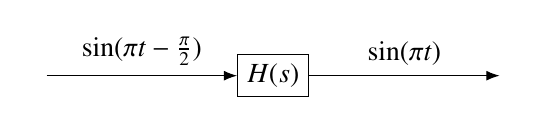
\begin{tikzpicture}[auto, node distance=4cm,>={Latex}]
  % Define blocks
  \node (input) at (0,0) {};
  \node [draw, rectangle] (H) at (3,0) {$H(s)$};
  \node (output) at (6,0) {};

  % Connect blocks with right arrows
  \draw [->] (input) -- node[midway, above] {$\sin(\pi t - \frac{\pi}{2})$} (H);
  \draw [->] (H) -- node[midway, above] {$\sin(\pi t)$} (output);
\end{tikzpicture}

  \captionsetup{justification=centering, singlelinecheck=off}
  \caption{Block diagram of inverse System}
  \label{fig:tikz_circuit}
\end{figure}

\begin{figure}[htb]
  \centering
  \input{./tikz/fig2.tex}
  \captionsetup{justification=centering, singlelinecheck=off}
  \caption{Block diagram of the System}
  \label{fig:tikz_circuit}
\end{figure}

\begin{figure}[h]
  \centering
  \includegraphics[width=\columnwidth]{./figs/fig1.png} 
  \captionsetup{justification=centering}
  \caption{Plot of $x(t)$ and $y(t)$ taken from Python}
  \label{fig:your_label}
\end{figure}

\begin{figure}[h]
  \centering
  \includegraphics[width=\columnwidth]{./figs/fig2.png} 
  \captionsetup{justification=centering}
  \caption{Plot of $\abs{H(j\omega}$  taken from Python}
  \label{fig:your_label}
\end{figure}


 \end{document}
